Um den Algorithmus besser verstehen zu können werden die Rahmenbedingungenwie folgt formalisiert. Die Datenbank, besitzt $\mathbf{N}$ Elemente, wobei  $\mathbf{N = 2^n}$ entspricht. Den Datensätzen werden die Elementen $\mathbf{ \{ 0,1 \}^n}$ zugeordnet. Wenn $\mathbf{ n=2}$ entspräche, besäße die Datenbank folgende Elemente: $\mathbf{00,01,10,11}$. Das gesuchte Elemente wird als $\mathbf{\hat{x}}$ bezeichnet. Die Datenbank wird als eine Funktion $\mathbf{f \{ 0,1 \}^n  \rightarrow \{ 0,1 \}}$ mit folgender Eigenschaft umgesetzt: \\
$\mathbf{f(x) = \begin{cases}1 \quad f\ddot{u}r \,
		x = \hat x \\0 \quad sonst \end{cases} 
}$ 
\newline
\\
Ist die Eingabe in die Funktion das gesuchte Element, so gibt diese $\mathbf{1}$ zurück, in allen anderen Fällen $\mathbf{0}$. 
Mithilfe dieser Funktion wird das Quantenorakel. $\mathbf{U_f : | x,y \rangle \to |x,y \oplus f(x) \rangle}$ erstellt. Das Quantenorakel, negiert das Vorzeichen des gesuchten Elements. Diese Funktionsweise ist aus dem Deutsch-Jozsa Algorithmus bekannt

\subsection{Prinzip}
Der Grover Algrothmus lässt sich in drei Schritte aufteilen.
\begin{enumerate}
	\item \textbf{Superpositionen aufbauen}
	\\
	Im ersten Schritt werden alle Quantenbits in die Superposition gebracht.
	\item \textbf{Amplitudenveränderung durchführen} \emph{(Grover Iteration G)}
	\\
	Der zweite Schritt verändert die Amplituden der Elemente. Dabei wird die Amplitude des gesuchten Elementes erhöht und alle anderen verringert. Dieser Schritt wird auch \emph{Grover Iteration (G)} genannt und abhängig von der Anzahl der Elementen öfters wiederholt. Wie oft \emph{G} ausgeführt werden muss wird im Abschnitt \ref{sec:geoVer} erläutert.
	\item \textbf{Messen} 
	\\
	Im letzten Schritt werden die Quantenbits gemessen. Mit einer hohen Wahrscheinlichkeit kommt das gesuchte Element $\mathbf{\hat x}$ heraus.
\end{enumerate}

\subsubsection{Amplitudenveränderung}
Die Amplitudenveränderung besteht aus zwei Schritten. Beim ersten Schritt wird das Vorzeichen der Amplitude von $\mathbf{\hat x}$ negiert. Im zweiten Schritt wird die negative Amplitude ausgenutzt um diese zu verstärken. Dies passiert in dem alle Amplituden am Mittelwert aller Amplituden gespiegelt werden. 
\\ \\
\textbf{Negieren der Amplitude}
 \\
Um die Amplitude von $\mathbf{\hat x}$ zu negieren, wird ein Hilfsbit und das Quantenorakel benötigt. Das Hilfsbit wird in den Zustand $\mathbf{H|1\rangle}$ mithilfe eines Hadamar Gatters gebracht. Dadurch erhalten wird $\mathbf{|x\rangle \frac{1}{\sqrt 2}(|0\rangle - |1\rangle )}$. Anschließend wird das Quantenorakel angewendet und damit das Vorzeichen der Amplitude von $\mathbf{\hat{x}}$ negiert. Das Hilfsbit wird nun nicht mehr benötigt und kann in folgenden Berechnungen weggelassen werden. Dies lässt sich auch an der Abbildung \ref{fig:changeAmplitude} erkennen. Dort ist Anwendung des Quantenorakel und graphisch die Amplituden alle Elemente der Datenbank mit $\mathbf{N=4}$ vor und nach der Anwendung des Quantenorakels zu sehen.
\begin{figure}[hbtp]
	\centering
	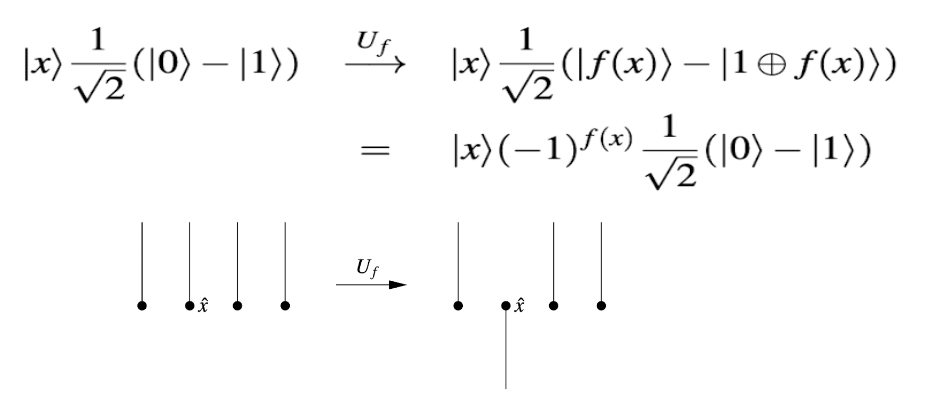
\includegraphics[width=.8\textwidth]{figures/amplitudenveraenderung.png}
	\caption{Amplitudenveränderung \\ Quelle: \cite[S. 141]{Ho17}}
	\label{fig:changeAmplitude}
\end{figure}
Die negative Amplitude von $\mathbf{\hat x}$ hat keinen Einfluss auf das Messen, um mit einer erhöhten Wahrscheinlichkeit das Element $\mathbf{\hat x}$ nach dem Messen zu erhalten wird Schritt zwei benötigt.
\\\\
\textbf{Spiegelung am Mittelwert} \\
\label{sec:spiegelnAmMittelwert} 
\noindent
Um zu zeigen, das die Spiegelung der Amplituden am Mittelwert den gewünschten Effekt hat, folgen nun ein paar Beispielrechnungen. Eine Spiegelung an einem wert $\mathbf{m}$ entspricht der Abbildung: $\mathbf{\alpha \rightarrow 2 \times m - \alpha}$. \\
Bei folgender Rechnung wird angenommen, dass die Datenbank vier Elemente enthält ($\mathbf{N=4}$). Der Mittelwert - nach der Negation von $\mathbf{\hat x}$ - hat den Wert: $\mathbf{m = \frac{1}{4} \times (\frac{1}{2}- \frac{1}{2}+ \frac{1}{2} +\frac{1}{2}) = \frac{1}{4}}$. Die Spiegelung von $\mathbf{\hat x}$ entspricht $\mathbf{-\frac{1}{2} \times \frac{1}{4} - (-\frac{1}{2}) = 1}$. Damit ist die Amplitude des gesuchten Elements gleich eins. Das Messen würde mit einer Wahrscheinlichkeit von 100\%  das gesuchte Element $\mathbf{\hat x}$ zurückgeben. Die Amplituden aller anderen Elemente entwickeln sich wie folgt: $\mathbf{\frac{1}{2} \times \frac{1}{4} - \frac{1}{2} = 0}$
\\ \\
Sei $\mathbf{N = 8}$, so würde die Amplitude von $\mathbf{ \hat x}$ nach der ersten Grover Iteration $\mathbf{\frac{5}{5\sqrt 8}}$ und alle anderen Amplituden $\mathbf{\frac{1}{2\sqrt 8}}$ betragen. Nach einer Spiegelung am Mittelwert ist die Amplituden von $\mathbf{\hat x}$ wieder positiv, bevor ein erneutes Spiegeln möglich ist, um die Amplitiduen weiter zu verstärken/verringern, muss erneut das Quantenorakel angewandt werden. Nach einer erneuten Negation und Spiegelung, hätte das gesuchte Element $\mathbf{\hat x}$ eine Amplitude von $\mathbf{0,973}$, alle anderen Elemente eine von $\mathbf{-0, 088}$. Würde nun gemessen werden erhielte man mit einer Wahrscheinlichkeit von 93 \% das gesuchte Element.
\\ 
Ein erneutes Spiegeln würde die Amplituden von $\mathbf{\hat{x}}$ im Gegensatz zu Erwartung wieder verringern und alle anderen erhöhen. Es ist daher besonders wichtig, dass nicht zu viele Grover Iterationen ausgeführt werden. Wie die Genaue Anzahl an Iterationen berechnet werden kann folgt im Abschnitt \ref{sec:geoVer}

\subsubsection{Graphische Darstellung des Grover Algorithmus}
Der Grover Algorithmus sieht nach dem bisherigen Erklärungen wie in Abbildung \ref{fig:algotInformellt} aus.
\begin{figure}[hbtp]
	\centering
	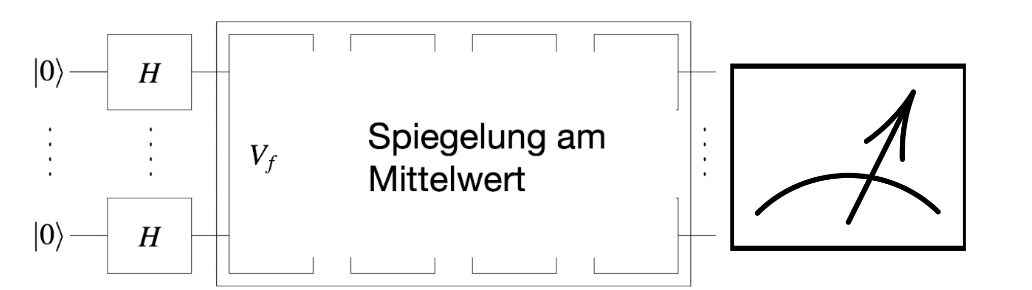
\includegraphics[width=1\textwidth]{figures/algoInformell.png}
	\caption{Graphische Darstellung des Grover Algorithmus \\ Quelle: Anlehnung an \cite[S. 146]{Ho17}}
	\label{fig:algoInformell}
\end{figure}
Alle QBits werden mithilfe der Hadamar Gatter in Superpositionen gebacht. Alles danach bis zum Messen Symbol am Ende der Abbildung ist die Grover Iteration.
Der Äußere Kasten steht in der Abbildung für das mehrfache Wiederholen der Grover-Iteration. $\mathbf{V_f}$ steht für das Quantenorakel, jedoch wird hier das Hilfsbit nicht mit eingezeichnet. Anschließend folgt die Spiegelung am Mittelwert. Wie diese genau mithilfe von Gattern umgesetzt wird, folgt im nächsten Abschnitt (\ref{sec:realiserung}). Nach dem ausführen der Grover Iterationen werden die QBits gemessen.
\subsection{Realisierung der Spiegelung am Mittelwert}
\label{sec:realiserung}
Die Abbildung $\mathbf{\alpha \rightarrow 2 \times m - \alpha}$ lässt sich mithilfe einer Matrixberechnung umsetzten.
\begin{center}
	$\mathbf{D_N \times 
	\begin{pmatrix}
			\alpha_0 \\ \alpha_1 \\ \vdots \\  \alpha_{N-1}
	\end{pmatrix}, \text{mit } D_N = 
	\begin{pmatrix}
			-1 + \frac{2}{N} & \frac{2}{N} & \dots& \frac{2}{N} \\
			\frac{2}{N} & -1 \frac{2}{N} & \dots& \frac{2}{N} \\
			\vdots & \vdots & \ddots& \dots \\
			 \frac{2}{N} & \frac{2}{N} & \dots& -1+ \frac{2}{N} \\
	\end{pmatrix}}$
\end{center}
\subsubsection{Beispielrechnung: Realisierung der Spiegelung am Mittelwert}
Sei $\mathbf{N = 4}$ so ergibt sich folgende Rechnung:
\begin{center}
 $\mathbf{D_4  \times \begin{pmatrix}
		0,5 & -0,5 & 0,5 & 0,5
\end{pmatrix}^T}$.

$\mathbf{\begin{pmatrix}
		-0,5 & 0,5 &0,5&0,5\\
		0,5 & -0,5 &0,5&0,5\\
		0,5 & 0,5 &-0,5&0,5\\
		0,5 & 0,5 &0,5&-0,5
	\end{pmatrix}
	\times \begin{pmatrix} 0,5 \\ -0,5 \\ 0,5 \\ 0,5 \end{pmatrix} = \begin{pmatrix} 0\\1\\0\\0 \end{pmatrix}
}$.
\end{center}
Dieses Ergebnis gleicht sich mit dem Ergebnis aus Abschnitt \ref{sec:spiegelnAmMittelwert}. In diesem wurden ebenfalls alle Elemente einer Datenbank mit $\mathbf{N=4}$ an dem Mittelwert der Amplituden gespiegelt. Folgende Abbildung \ref{fig:spiegelung} zeigt graphisch, wie sich die Amplituden verändert haben.
\begin{figure}[hbtp]
	\centering
	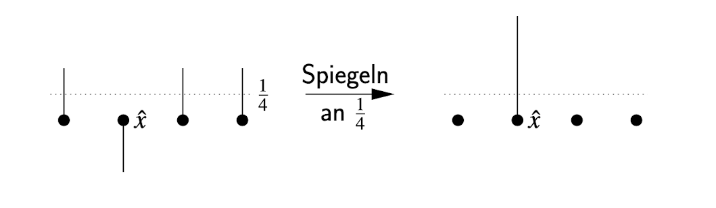
\includegraphics[width=.8\textwidth]{figures/spiegelung.png}
	\caption{Spiegelung am Mittelwert \\ Quelle: \cite[S. 142]{Ho17}}
	\label{fig:spiegelung}
\end{figure}
\noindent
\\
Wenn eine $\mathbf{N \times N}$ Matrix verwendet wird, dann verstößt dies gegen das Lokalitätsprinzip. Daher muss die $\mathbf{D_n}$ Matrix in verschiedene unitäre Matrizen zerlegt werden.  $\mathbf{D_n}$ kann in ein Produkt aus drei unitäre Matrizen zerlegt werden.
\begin{center}
$\mathbf{D_n = -H_n \times R_N \times H_n, \text{mit } R  = 
\begin{pmatrix}
		-1 & 0 &\dots& 0 \\
		0& 1& \ddots& \vdots\\
		\vdots &\ddots& \ddots&0 \\
		0& \dots& 0 &1 \\
\end{pmatrix}}$
\end{center}
\subsubsection{Beispielrechnung: Realisierung der Spiegelung am Mittelwert  mithilfe von unitären Matrizen}
Um zu zeigen das die Matrix $\mathbf{D_N}$ wie oben abgebildet als Produkt von drei Matrizen zerlegt werden kann, folgt ein Beispiel mit $\mathbf{N = 4}$.
\begin{figure}[hbtp]
	\centering
	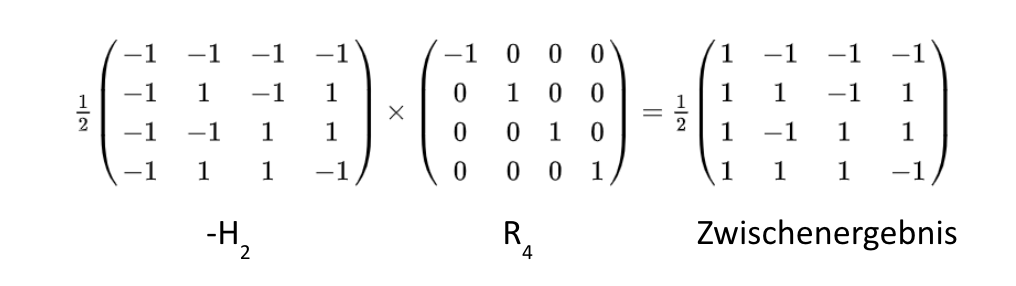
\includegraphics[width=.8\textwidth]{figures/householderLokal_1.png}
	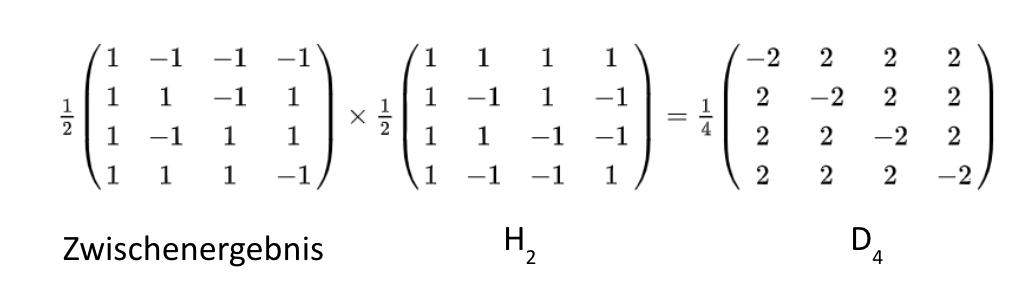
\includegraphics[width=.8\textwidth]{figures/householderLokal_2.png}
	\caption{Beispielzerlegung von $\mathbf{D_4}$ \\ Quelle: Eigene Darstellung}
	\label{fig:DLokal}
\end{figure}
Das Ergebnis der Berechnung ist, wie in der beschriftetet Rechnung \ref{fig:DLokal} zu sehen, gleich mit der zu erwarteten Matrix $\mathbf{D_4}$. Der Beweis, das dies auch für beliebige $\mathbf{N}$ zutrifft, befindet sich in dem Buch vom M. Hoemeister \cite[S. 309]{Ho17}.

\subsubsection{Matrix R als lokale Transformation}
Es wurde gezeigt das die Matrix $\mathbf{D_N}$ in ein Produkt aus Matrizen zerlegt werden kann. Das die Hadamar Matrix mit Hilfe eines Gatters als lokale Transformation umgesetzt werden kann, ist bekannt. Dies muss jedoch auch noch für $\mathbf{R_N}$ gezeigt werden. 
\\
Um ein Gatter zu entwickeln zu können, welches die Transformation $\mathbf{R_N}$ umsetzt, muss verstanden werden, wie sich $\mathbf{R_N}$ bei einer Multiplikation von Matrizen auswirkt. Alle Werte einer Matrix die mit $\mathbf{R_N}$ multipliziert wird bleiben gleich. Lediglich die erste Zeile oder Spalte wird negiert. Dies ist davon abhängig, ob die Matrix $\mathbf{R_N}$ auf der Linken oder Rechten Seite der Multiplikation steht. In ersten Zeile der Abbildung \ref{fig:DLokal} ist die Negation der ersten Spalte zu sehen.
\\
Multipliziert man $\mathbf{R_N}$ mit Amplituden, bedeutet dies, dass lediglich die Amplitude des ersten Elementes ($\mathbf{|0...0\rangle}$) negiert wird.
Die Abbildung \ref{fig:Rgatter} zeigt den Quantenschaltkreis, wenn $\mathbf{N = 4}$ gilt.
 \begin{figure}[hbtp]
 	\centering
 	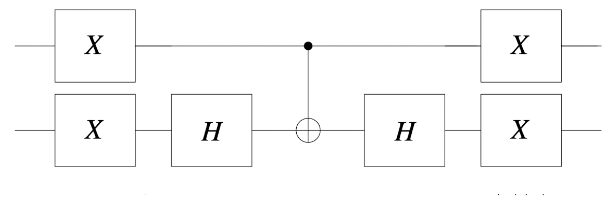
\includegraphics[width=.8\textwidth]{figures/rgatter.png}
 	\caption{$\mathbf{R_4}$ Realisierung \\ Quelle: \cite[S. 145]{Ho17}}
 	\label{fig:Rgatter}
 \end{figure}
\\
Es folgen weitere Beispielrechnungen, um zu verdeutlichen, dass der Quantenschaltkreis die Transformation $\mathbf{R_4}$ ausführt.
\subsubsection{Beispielrechnung: Matrix R als lokale Transformation}
 \begin{figure}[hbtp]
	\centering
	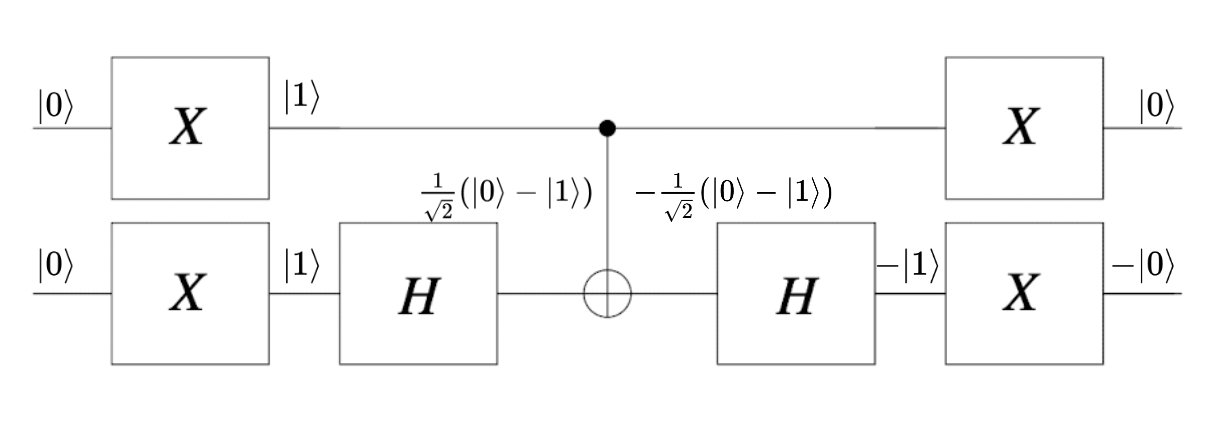
\includegraphics[width=.8\textwidth]{figures/RGatter00.png}
	\caption{$\mathbf{|00\rangle}$ Werteveränderungen durch das$\mathbf{R_4}$-Gatter \\ Quelle: Anlehnung an \cite[S. 145]{Ho17}}
	\label{fig:Rgatter00}
\end{figure}
 In den Abbildungen \ref{fig:Rgatter00} werden die Werte der QBits $\mathbf{|00\rangle}$ und wie diese sich durch die einzelnen Gatter verändern dargestellt.
 Die Pauli X-Gatter invertieren den Wert eines QBits. Aus $\mathbf{|0\rangle}$ wird $\mathbf{|1\rangle}$ und andersherum. Das erste Bit wird bis zum letzten Pauli-X Gatter nicht mehr verändert. Es wird ausschließlich genutzt um zu schauen, ob das CNOT aktiviert wird. Das zweite QBit wird durch das erste Hadamar Gatter, in folgende Superposition $\mathbf{\frac{1}{\sqrt 2}(|0\rangle - |1\rangle)}$ gebracht. Da das erste QBit den Wert $\mathbf{|1\rangle}$ hat wird das zweite QBit durch das CNOT negiert, und hat den Wert: - $\mathbf{-\frac{1}{\sqrt 2}(|0\rangle - |1\rangle)}$. Anschließend durch läuft das zweite Bit wieder ein Hadamar Gatter. Das QBit hat anschließend folgenden Wert: $\mathbf{-|1\rangle}$.
 Zum Schluss werden beide Bits ($\mathbf{|1\rangle}$ und $\mathbf{-|1\rangle}$) durch die Pauli-X Gatter invertiert und wir erhalten das gewünschte und erwartete Ergebnis $\mathbf{-|00\rangle}$.
  \\
  \\
   \begin{figure}[hbtp]
  	\centering
  	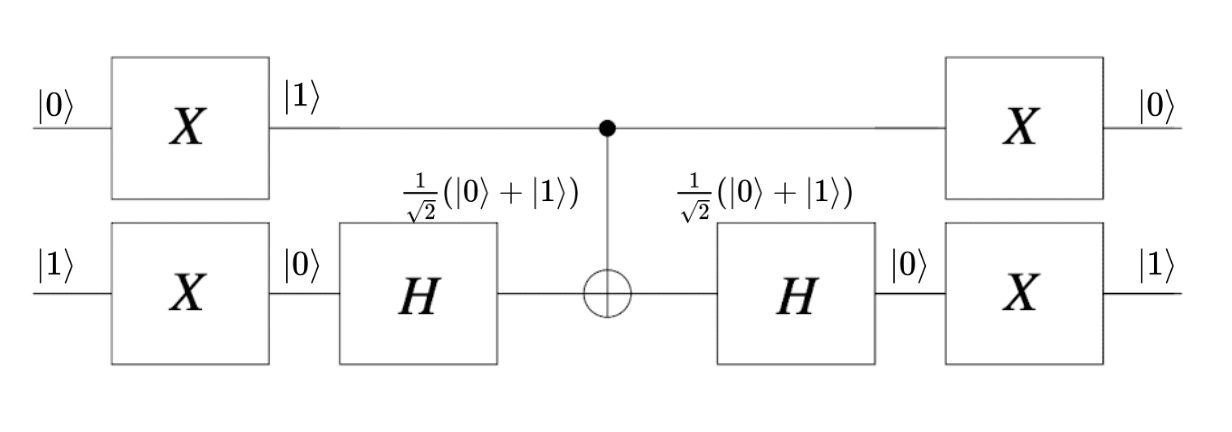
\includegraphics[width=.8\textwidth]{figures/RGatter01.png}
  	\caption{$|00\rangle$ Werte Veränderungen durch das $R_4$-Gatter \\ Quelle: Anlehnung an \cite[S. 145]{Ho17}}
  	\label{fig:Rgatter01}
  \end{figure}
\noindent
 Die Abbildung \ref{fig:Rgatter01} zeigt die QBits $\mathbf{|01\rangle}$  und wie diese von den Gattern verändert werden. Die ersten Pauli-X Gatter invertieren abermals die QBits, diese haben nun den Wert $\mathbf{|10\rangle}$. Das erste QBit wird bis auf von dem letzten Pauli-X Gatter nicht verändert und nur zur Aktivierung der Operation CNOT zuhilfe genommen. Das zweite QBit wird durch das Hadamar Gatter in die Superpostion $\mathbf{\frac{1}{\sqrt 2}(|0\rangle + |1\rangle)}$ gebracht. Diese verändert sich nicht durch die CNOT Operation. Nach der CNOT Operation wird das QBit durch das zweite Hadamar Gatter wieder in den Basiszustand $\mathbf{|0\rangle}$ gebracht. Zuletzt durchlaufen die beiden QBits ein Pauli-X Gatter welches die QBits von den Basiszustände $\mathbf{|10\rangle}$ in den erwarteten Zustand $\mathbf{|01\rangle}$ überführt. Die QBits haben wie erwartet, nach dem durchlaufen des Quantenschaltkreises die selben Zustände wie vorher.
  \\ 
  \\
Bei den QBits $\mathbf{|10\rangle \text{ und }|11\rangle}$, wird die CNOT Operation nicht ausgeführt, da das erste QBit in den Basiszustand $\mathbf{|0\rangle}$ überführt werden. Die QBits werden durch die doppelte Ausführung der Gatter ebenfalls nicht verändert. Aus diesen Gründen ist für diese beiden Beispiel keine Abbildung vorhanden.
\\
\\
An den Beispielen kann gesehen werden, dass der Quantenschaltkreis die gewünschte Operation $\mathbf{R_4}$ ausführen.

\subsection{Graphische Darstellung des Grover Algorithmus}
In der Abbildung \ref{fig:algoFormell} ist wie in der Abbildung \ref{fig:algoInformell} der Grover Algorithmus Graphisch dargestellt. Die Abbildung enthält alle Gatter die für den Grover Algorithmus benötigt werden. Hilfbits sind hier ebenfalls nicht eingezeichnet.
\begin{figure}[hbtp]
	\centering
	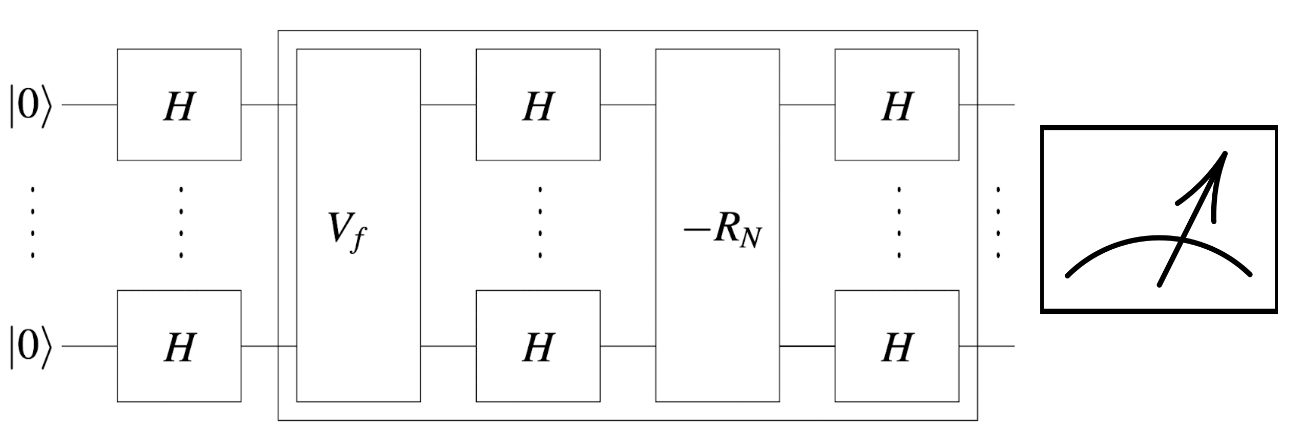
\includegraphics[width=1\textwidth]{figures/algoFormell.png}
	\caption{Graphische Darstellung des Grover Algorithmus \\ Quelle: Anlehnung an \cite[S. 146]{Ho17} }
	\label{fig:algoFormell}
\end{figure}



